\upaper{114}{Seraphic Planetary Government}
\author{Chief of Seraphim}
\vs p114 0:1 The Most Highs rule in the kingdoms of men through many celestial forces and agencies but chiefly through the ministry of seraphim.
\vs p114 0:2 At noon today the roll call of planetary angels, guardians, and others on Urantia was 501,234,619 pairs of seraphim. There were assigned to my command 200 seraphic hosts --- 597,196,800 pairs of seraphim, or 1,194,393,600 individual angels. The registry, however, shows 1,002,469,238 individuals; it follows therefore that 191,924,362 angels were absent from this world on transport, messenger, and death duty. (On Urantia there are about the same number of cherubim as seraphim, and they are similarly organized.)
\vs p114 0:3 Seraphim and their associated cherubim have much to do with the details of the superhuman government of a planet, especially of worlds which have been isolated by rebellion. The angels, ably assisted by the midwayers, function on Urantia as the actual supermaterial ministers who execute the mandates of the resident governor general and all his associates and subordinates. Seraphim as a class are occupied with many assignments other than those of personal and group guardianship.
\vs p114 0:4 Urantia is not without proper and effective supervision from the system, constellation, and universe rulers. But the planetary government is unlike that of any other world in the Satania system, even in all Nebadon. This uniqueness in your plan of supervision is due to a number of unusual circumstances:
\vs p114 0:5 \ublistelem{1.}\bibnobreakspace The life modification status of Urantia.
\vs p114 0:6 \ublistelem{2.}\bibnobreakspace The exigencies of the Lucifer rebellion.
\vs p114 0:7 \ublistelem{3.}\bibnobreakspace The disruptions of the Adamic default.
\vs p114 0:8 \ublistelem{4.}\bibnobreakspace The irregularities growing out of the fact that Urantia was one of the bestowal worlds of the Universe Sovereign. Michael of Nebadon is the Planetary Prince of Urantia.
\vs p114 0:9 \ublistelem{5.}\bibnobreakspace The special function of the 24 planetary directors.
\vs p114 0:10 \ublistelem{6.}\bibnobreakspace The location on the planet of an archangels’ circuit.
\vs p114 0:11 \ublistelem{7.}\bibnobreakspace The more recent designation of the onetime incarnated Machiventa Melchizedek as vicegerent Planetary Prince.
\usection{1.\bibnobreakspace The Sovereignty of Urantia}
\vs p114 1:1 The original sovereignty of Urantia was held in trust by the sovereign of the Satania system. It was first delegated by him to a joint commission of Melchizedeks and Life Carriers, and this group functioned on Urantia until the arrival of a regularly constituted Planetary Prince. Subsequent to the downfall of Prince Caligastia, at the time of the Lucifer rebellion, Urantia had no sure and settled relationship with the local universe and its administrative divisions until the completion of Michael’s bestowal in the flesh, when he was proclaimed, by the Union of Days, Planetary Prince of Urantia. Such a proclamation in surety and in principle forever settled the status of your world, but in practice the Sovereign Creator Son made no gesture of personal administration of the planet aside from the establishment of the Jerusem commission of 24 former Urantians with authority to represent him in the government of Urantia and all other quarantined planets in the system. One of this council is now always resident on Urantia as resident governor general.
\vs p114 1:2 Vicegerent authority to act for Michael as Planetary Prince has been recently vested in Machiventa Melchizedek, but this Son of the local universe has made not the slightest move toward modifying the present planetary regime of the successive administrations of the resident governors general.
\vs p114 1:3 There is little likelihood that any marked change will be made in the government of Urantia during the present dispensation unless the vicegerent Planetary Prince should arrive to assume his titular responsibilities. It appears to certain of our associates that at some time in the near future the plan of sending one of the 24 counsellors to Urantia to act as governor general will be superseded by the formal arrival of Machiventa Melchizedek with the vicegerent mandate of the sovereignty of Urantia. As acting Planetary Prince he would undoubtedly continue in charge of the planet until the final adjudication of the Lucifer rebellion and probably on into the distant future of planetary settlement in light and life.
\vs p114 1:4 Some believe that Machiventa will not come to take personal direction of Urantian affairs until the end of the current dispensation. Others hold that the vicegerent Prince may not come, as such, until Michael sometime returns to Urantia as he promised when still in the flesh. Still others, including this narrator, look for Melchizedek’s appearance any day or hour.
\usection{2.\bibnobreakspace The Board of Planetary Supervisors}
\vs p114 2:1 Since the times of Michael’s bestowal on your world the general management of Urantia has been entrusted to a special group on Jerusem of 24 onetime Urantians. Qualification for membership on this commission is unknown to us, but we have observed that those who have been thus commissioned have all been contributors to the enlarging sovereignty of the Supreme in the system of Satania. By nature they were all real leaders when they functioned on Urantia, and (excepting Machiventa Melchizedek) these qualities of leadership have been further augmented by mansion world experience and supplemented by the training of Jerusem citizenship. Members are nominated to the 24 by the cabinet of Lanaforge, seconded by the Most Highs of Edentia, approved by the Assigned Sentinel of Jerusem, and appointed by Gabriel of Salvington in accordance with the mandate of Michael. The temporary appointees function just as fully as do the permanent members of this commission of special supervisors.
\vs p114 2:2 This board of planetary directors is especially concerned with the supervision of those activities on this world which result from the fact that Michael here experienced his terminal bestowal. They are kept in close and immediate touch with Michael by the liaison activities of a certain Brilliant Evening Star, the identical being who attended upon Jesus throughout the mortal bestowal.
\vs p114 2:3 At the present time one John, known to you as “the Baptist,” is chairman of this council when it is in session on Jerusem. But the ex officio head of this council is the Assigned Sentinel of Satania, the direct and personal representative of the Associate Inspector on Salvington and of the Supreme Executive of Orvonton.
\vs p114 2:4 The members of this same commission of former Urantians also act as advisory supervisors of the 36 other rebellion\hyp{}isolated worlds of the system; they perform a very valuable service in keeping Lanaforge, the System Sovereign, in close and sympathetic touch with the affairs of these planets, which still remain more or less under the overcontrol of the Constellation Fathers of Norlatiadek. These 24 counsellors make frequent trips as individuals to each of the quarantined planets, especially to Urantia.
\vs p114 2:5 Each of the other isolated worlds is advised by similar and varying sized commissions of its onetime inhabitants, but these other commissions are subordinate to the Urantian group of 24. While the members of the latter commission are thus actively interested in every phase of human progress on each quarantined world in Satania, they are especially and particularly concerned with the welfare and advancement of the mortal races of Urantia, for they immediately and directly supervise the affairs of none of the planets except Urantia, and even here their authority is not complete excepting in certain domains concerned with mortal survival.
\vs p114 2:6 No one knows how long these 24 Urantia counsellors will continue in their present status, detached from the regular program of universe activities. They will no doubt continue to serve in their present capacities until some change in planetary status ensues, such as the end of a dispensation, the assumption of full authority by Machiventa Melchizedek, the final adjudication of the Lucifer rebellion, or the reappearance of Michael on the world of his final bestowal. The present resident governor general of Urantia seems inclined to the opinion that all but Machiventa may be released for Paradise ascension the moment the system of Satania is restored to the constellation circuits. But other opinions are also current.
\usection{3.\bibnobreakspace The Resident Governor General}
\vs p114 3:1 Every 100 years of Urantia time, the Jerusem corps of 24 planetary supervisors designate one of their number to sojourn on your world to act as their executive representative, as resident governor general. During the times of the preparation of these narratives this executive officer was changed, the 19\ts{th} so to serve being succeeded by the 20\ts{th}. The name of the current planetary supervisor is withheld from you only because mortal man is so prone to venerate, even to deify, his extraordinary compatriots and superhuman superiors.
\vs p114 3:2 The resident governor general has no actual personal authority in the management of world affairs except as the representative of the 24 Jerusem counsellors. He acts as the co\hyp{}ordinator of superhuman administration and is the respected head and universally recognized leader of the celestial beings functioning on Urantia. All orders of angelic hosts regard him as their co\hyp{}ordinating director, while the United Midwayers\fnc{\textbf{United Midwayers}, In 1955 text: united midwayers.}, since the departure of 1\hyp{}2\hyp{}3 the first to become one of the 24 counsellors, really look upon the successive governors general as their planetary fathers.
\vs p114 3:3 Although the governor general does not possess actual and personal authority on the planet, he hands down scores of rulings and decisions each day which are accepted as final by all personalities concerned. He is much more of a fatherly adviser than a technical ruler. In certain ways he functions as would a Planetary Prince, but his administration much more closely resembles that of the Material Sons.
\vs p114 3:4 \pc The Urantia government is represented in the councils of Jerusem in accordance with an arrangement whereby the returning governor general sits as a temporary member of the System Sovereign’s cabinet of Planetary Princes. It was expected, when Machiventa was designated vicegerent Prince, that he would immediately assume his place in the council of the Planetary Princes of Satania, but thus far he has made no gesture in this direction.
\vs p114 3:5 The supermaterial government of Urantia does not maintain a very close organic relationship with the higher units of the local universe. In a way, the resident governor general represents Salvington as well as Jerusem since he acts on behalf of the 24 counsellors, who are directly representative of Michael and Gabriel. And being a Jerusem citizen, the planetary governor can function as a spokesman for the System Sovereign. The constellation authorities are represented directly by a Vorondadek Son, the Edentia observer.
\usection{4.\bibnobreakspace The Most High Observer}
\vs p114 4:1 The sovereignty of Urantia is further complicated by the onetime arbitrary seizure of planetary authority by the government of Norlatiadek shortly after the planetary rebellion. There is still resident on Urantia a Vorondadek Son, an observer for the Most Highs of Edentia and, in the absence of direct action by Michael, trustee of planetary sovereignty. The present Most High observer (and sometime regent) is the 23\ts{rd} thus to serve on Urantia.
\vs p114 4:2 There are certain groups of planetary problems which are still under the control of the Most Highs of Edentia, jurisdiction over them having been seized at the time of the Lucifer rebellion. Authority in these matters is exercised by a Vorondadek Son, the Norlatiadek observer, who maintains very close advisory relations with the planetary supervisors. The race commissioners are very active on Urantia, and their various group chiefs are informally attached to the resident Vorondadek observer, who acts as their advisory director.
\vs p114 4:3 In a crisis the actual and sovereign head of the government, excepting in certain purely spiritual matters, would be this Vorondadek Son of Edentia now on observation duty. (In these exclusively spiritual problems and in certain purely personal matters, the supreme authority seems to be vested in the commanding archangel attached to the divisional headquarters of that order which was recently established on Urantia.)
\vs p114 4:4 \pc A Most High observer is empowered, at his discretion, to seize the planetary government in times of grave planetary crises, and it is of record that this has happened 33 times in the history of Urantia. At such times the Most High observer functions as the Most High regent, exercising unquestioned authority over all ministers and administrators resident on the planet excepting only the divisional organization of the archangels.
\vs p114 4:5 Vorondadek regencies are not peculiar to rebellion\hyp{}isolated planets, for the Most Highs may intervene at any time in the affairs of the inhabited worlds, interposing the superior wisdom of the constellation rulers in the affairs of the kingdoms of men.
\usection{5.\bibnobreakspace The Planetary Government}
\vs p114 5:1 The actual administration of Urantia is indeed difficult to describe. There exists no formal government along the lines of universe organization, such as separate legislative, executive, and judicial departments. The 24 counsellors come the nearest to being the legislative branch of the planetary government. The governor general is a provisional and advisory chief executive with the veto power resident in the Most High observer. And there are no absolutely authoritative judicial powers operative on the planet --- only the conciliating commissions.
\vs p114 5:2 A majority of the problems involving seraphim and midwayers are, by mutual consent, decided by the governor general. But except when voicing the mandates of the 24 counsellors, his rulings are all subject to appeal to conciliating commissions, to local authorities constituted for planetary function, or even to the System Sovereign of Satania.
\vs p114 5:3 The absence of the corporeal staff of a Planetary Prince and the material regime of an Adamic Son and Daughter is partially compensated by the special ministry of seraphim and by the unusual services of the midway creatures. The absence of the Planetary Prince is effectively compensated by the triune presence of the archangels, the Most High observer, and the governor general.
\vs p114 5:4 This rather loosely organized and somewhat personally administered planetary government is more than expectedly effective because of the timesaving assistance of the archangels and their ever\hyp{}ready circuit, which is so frequently utilized in planetary emergencies and administrative difficulties. Technically, the planet is still spiritually isolated in the Norlatiadek circuits, but in an emergency this handicap can now be circumvented through utilization of the archangels’ circuit. Planetary isolation is, of course, of little concern to individual mortals since the pouring out of the Spirit of Truth upon all flesh 1900 years ago.
\vs p114 5:5 \pc Each administrative day on Urantia begins with a consultative conference, which is attended by the governor general, the planetary chief of archangels, the Most High observer, the supervising supernaphim, the chief of resident Life Carriers, and invited guests from among the high Sons of the universe or from among certain of the student visitors who may chance to be sojourning on the planet.
\vs p114 5:6 The direct administrative cabinet of the governor general consists of 12 seraphim, the acting chiefs of the 12 groups of special angels functioning as the immediate superhuman directors of planetary progress and stability.
\usection{6.\bibnobreakspace The Master Seraphim of Planetary Supervision}
\vs p114 6:1 When the first governor general arrived on Urantia, concurrent with the outpouring of the Spirit of Truth, he was accompanied by 12 corps of special seraphim, Seraphington graduates, who were immediately assigned to certain special planetary services. These exalted angels are known as the master seraphim of planetary supervision and are, aside from the overcontrol of the planetary Most High observer, under the immediate direction of the resident governor general.
\vs p114 6:2 These 12 groups of angels, while functioning under the general supervision of the resident governor general, are immediately directed by the seraphic council of 12, the acting chiefs of each group. This council also serves as the volunteer cabinet of the resident governor general.
\vs p114 6:3 As planetary chief of seraphim, I preside over this council of seraphic chiefs, and I am a volunteer supernaphim of the primary order serving on Urantia as the successor of the onetime chief of the angelic hosts of the planet who defaulted at the time of the Caligastia secession.
\vs p114 6:4 The 12 corps of the master seraphim of planetary supervision are functional on Urantia as follows:
\vs p114 6:5 \ublistelem{1.}\bibnobreakspace \bibemph{The epochal angels.} These are the angels of the current age, the dispensational group. These celestial ministers are entrusted with the oversight and direction of the affairs of each generation as they are designed to fit into the mosaic of the age in which they occur. The present corps of epochal angels serving on Urantia is the third group assigned to the planet during the current dispensation.
\vs p114 6:6 \ublistelem{2.}\bibnobreakspace \bibemph{The progress angels.} These seraphim are entrusted with the task of initiating the evolutionary progress of the successive social ages. They foster the development of the inherent progressive trend of evolutionary creatures; they labour incessantly to make things what they ought to be. The group now on duty is the second to be assigned to the planet.
\vs p114 6:7 \ublistelem{3.}\bibnobreakspace \bibemph{The religious guardians.} These are the “angels of the churches,” the earnest contenders for that which is and has been. They endeavour to maintain the ideals of that which has survived for the sake of the safe transit of moral values from one epoch to another. They are the checkmates of the angels of progress, all the while seeking to translate from one generation to another the imperishable values of the old and passing forms into the new and therefore less stabilized patterns of thought and conduct. These angels do contend for spiritual forms, but they are not the source of ultrasectarianism and meaningless controversial divisions of professed religionists. The corps now functioning on Urantia is the fifth thus to serve.
\vs p114 6:8 \ublistelem{4.}\bibnobreakspace \bibemph{The angels of nation life.} These are the “angels of the trumpets,” directors of the political performances of Urantia national life. The group now functioning in the overcontrol of international relations is the fourth corps to serve on the planet. It is particularly through the ministry of this seraphic division that “the Most Highs rule in the kingdoms of men.”
\vs p114 6:9 \ublistelem{5.}\bibnobreakspace \bibemph{The angels of the races.} Those who work for the conservation of the evolutionary races of time, regardless of their political entanglements and religious groupings. On Urantia there are remnants of nine human races which have commingled and combined into the people of modern times. These seraphim are closely associated with the ministry of the race commissioners, and the group now on Urantia is the original corps assigned to the planet soon after the day of Pentecost.
\vs p114 6:10 \ublistelem{6.}\bibnobreakspace \bibemph{The angels of the future.} These are the projection angels, who forecast a future age and plan for the realization of the better things of a new and advancing dispensation; they are the architects of the successive eras. The group now on the planet has thus functioned since the beginning of the current dispensation.
\vs p114 6:11 \ublistelem{7.}\bibnobreakspace \bibemph{The angels of enlightenment.} Urantia is now receiving the help of the third corps of seraphim dedicated to the fostering of planetary education. These angels are occupied with mental and moral training as it concerns individuals, families, groups, schools, communities, nations, and whole races.
\vs p114 6:12 \ublistelem{8.}\bibnobreakspace \bibemph{The angels of health.} These are the seraphic ministers assigned to the assistance of those mortal agencies dedicated to the promotion of health and the prevention of disease. The present corps is the sixth group to serve during this dispensation.
\vs p114 6:13 \ublistelem{9.}\bibnobreakspace \bibemph{The home seraphim.} Urantia now enjoys the services of the fifth group of angelic ministers dedicated to the preservation and advancement of the home, the basic institution of human civilization.
\vs p114 6:14 \ublistelem{10.}\bibnobreakspace \bibemph{The angels of industry.} This seraphic group is concerned with fostering industrial development and improving economic conditions among the Urantia peoples. This corps has been seven times changed since the bestowal of Michael.
\vs p114 6:15 \ublistelem{11.}\bibnobreakspace \bibemph{The angels of diversion.} These are the seraphim who foster the values of play, humour, and rest. They ever seek to uplift man’s recreational diversions and thus to promote the more profitable utilization of human leisure. The present corps is the third of that order to minister on Urantia.
\vs p114 6:16 \ublistelem{12.}\bibnobreakspace \bibemph{The angels of superhuman ministry.} These are the angels of the angels, those seraphim who are assigned to the ministry of all other superhuman life on the planet, temporary or permanent. This corps has served since the beginning of the current dispensation.\tunemarkup{pictures}{\begin{figure}[H]\centering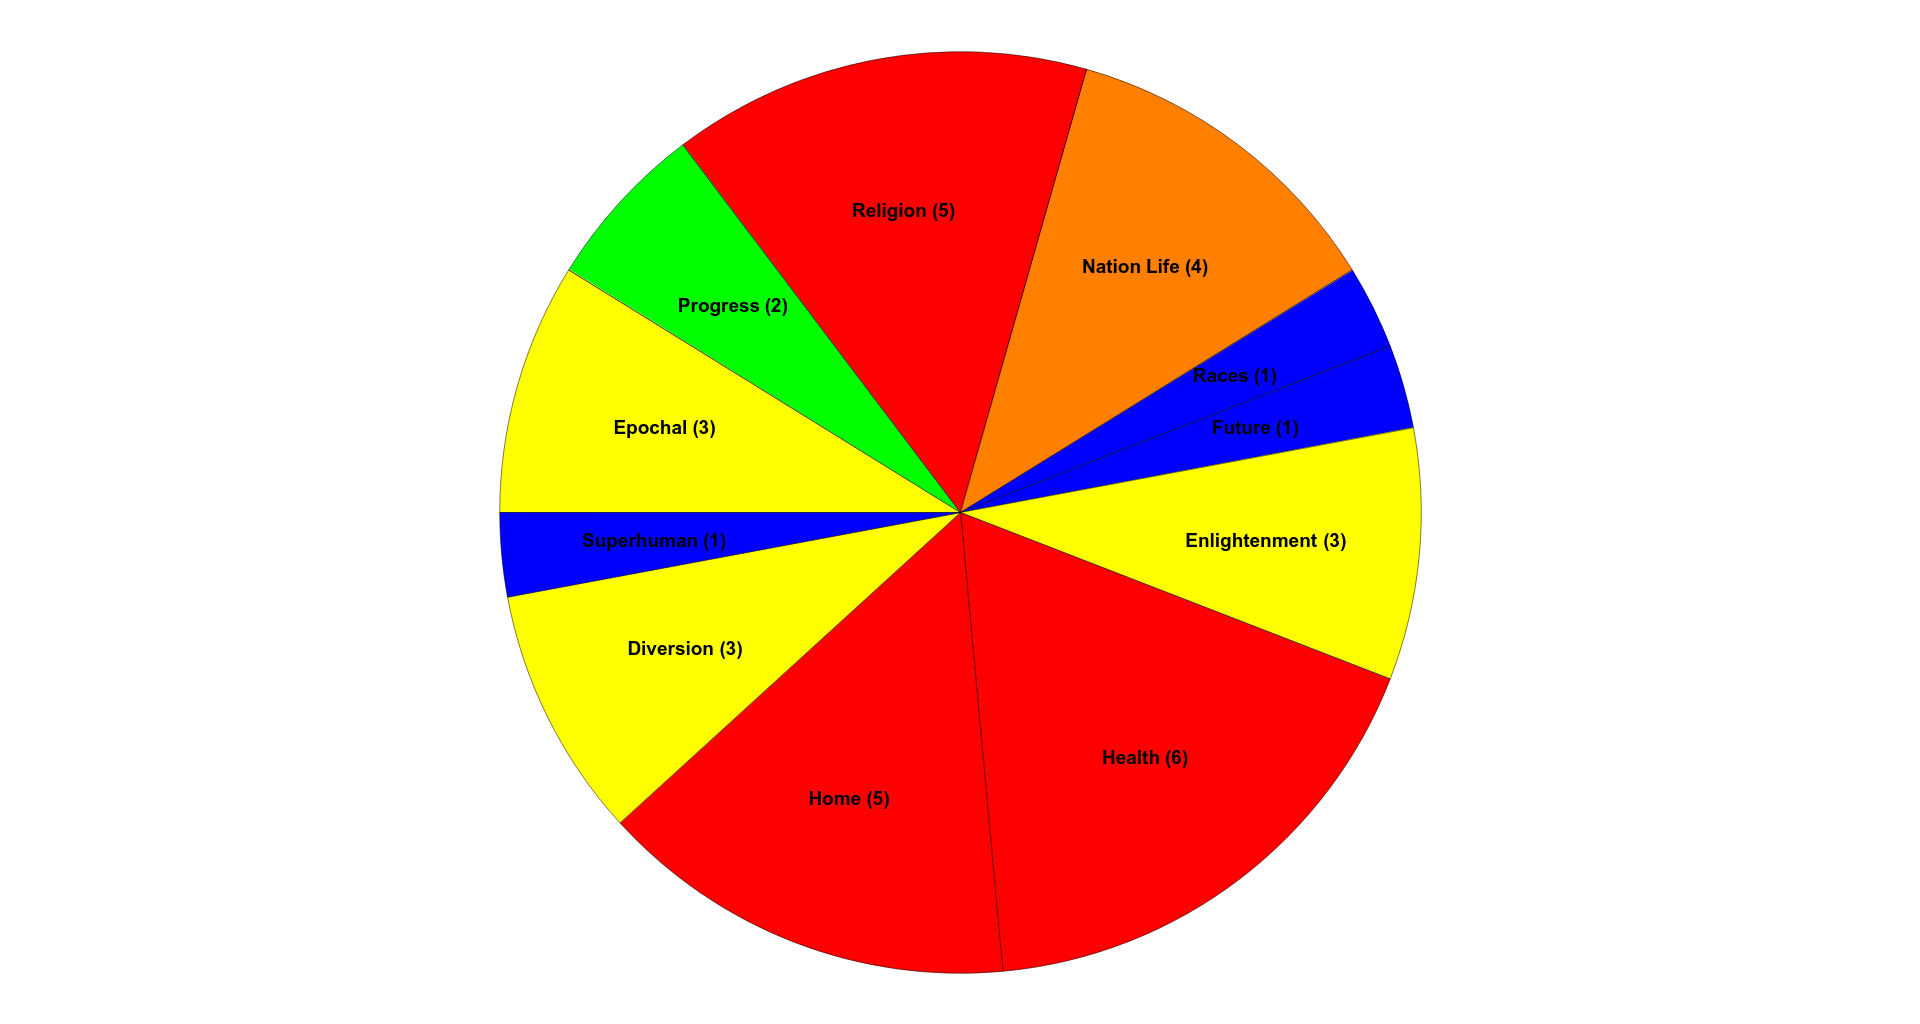
\includegraphics[width=1.3\columnwidth]{images/angelic-corps.png}\caption{Performance of the Angelic Corps.}\end{figure}}
\vs p114 6:17 \pc When these groups of master seraphim disagree in matters of planetary policy or procedure, their differences are usually composed by the governor general, but all his rulings are subject to appeal in accordance with the nature and gravity of the issues involved in the disagreement.
\vs p114 6:18 None of these angelic groups exercise direct or arbitrary control over the domains of their assignment. They cannot fully control the affairs of their respective realms of action, but they can and do so manipulate planetary conditions and so associate circumstances as favourably to influence the spheres of human activity to which they are attached.
\vs p114 6:19 The master seraphim of planetary supervision utilize many agencies for the prosecution of their missions. They function as ideational clearinghouses, mind focalizers, and project promoters. While unable to inject new and higher conceptions into human minds, they often act to intensify some higher ideal which has already appeared within a human intellect.
\vs p114 6:20 But aside from these many means of positive action, the master seraphim insure planetary progress against vital jeopardy through the mobilization, training, and maintenance of the reserve corps of destiny. The chief function of these reservists is to insure against breakdown of evolutionary progress; they are the provisions which the celestial forces have made against surprise; they are the guarantees against disaster.
\usection{7.\bibnobreakspace The Reserve Corps of Destiny}
\vs p114 7:1 The reserve corps of destiny consists of living men and women who have been admitted to the special service of the superhuman administration of world affairs. This corps is made up of the men and women of each generation who are chosen by the spirit directors of the realm to assist in the conduct of the ministry of mercy and wisdom to the children of time on the evolutionary worlds. It is the general practice in the conduct of the affairs of the ascension plans to begin this liaison utilization of mortal will creatures immediately they are competent and trustworthy to assume such responsibilities. Accordingly, as soon as men and women appear on the stage of temporal action with sufficient mental capacity, adequate moral status, and requisite spirituality, they are quickly assigned to the appropriate celestial group of planetary personalities as human liaisons, mortal assistants.
\vs p114 7:2 When human beings are chosen as protectors of planetary destiny, when they become pivotal individuals in the plans which the world administrators are prosecuting, at that time the planetary chief of seraphim confirms their temporal attachment to the seraphic corps and appoints personal destiny guardians to serve with these mortal reservists. All reservists have self\hyp{}conscious Adjusters, and most of them function in the higher cosmic circles of intellectual achievement and spiritual attainment.
\vs p114 7:3 Mortals of the realm are chosen for service in the reserve corps of destiny on the inhabited worlds because of:
\vs p114 7:4 \ublistelem{1.}\bibnobreakspace Special capacity for being secretly rehearsed for numerous possible emergency missions in the conduct of various activities of world affairs.
\vs p114 7:5 \ublistelem{2.}\bibnobreakspace Wholehearted dedication to some special social, economic, political, spiritual, or other cause, coupled with willingness to serve without human recognition and rewards.
\vs p114 7:6 \ublistelem{3.}\bibnobreakspace The possession of a Thought Adjuster of extraordinary versatility and probable pre\hyp{}Urantia experience in coping with planetary difficulties and contending with impending world emergency situations.
\vs p114 7:7 \pc Each division of planetary celestial service is entitled to a liaison corps of these mortals of destiny standing. The average inhabited world employs 70 separate corps of destiny, which are intimately connected with the superhuman current conduct of world affairs. On Urantia there are 12 reserve corps of destiny, one for each of the planetary groups of seraphic supervision.
\vs p114 7:8 The 12 groups of Urantia destiny reservists are composed of mortal inhabitants of the sphere who have been rehearsed for numerous crucial positions on earth and are held in readiness to act in possible planetary emergencies. This combined corps now consists of 962 persons. The smallest corps numbers 41 and the largest 172. With the exception of less than a score of contact personalities, the members of this unique group are wholly unconscious of their preparation for possible function in certain planetary crises. These mortal reservists are chosen by the corps to which they are respectively attached and are likewise trained and rehearsed in the deep mind by the combined technique of Thought Adjuster and seraphic guardian ministry. Many times numerous other celestial personalities participate in this unconscious training, and in all this special preparation the midwayers perform valuable and indispensable services.
\vs p114 7:9 On many worlds the better adapted secondary midway creatures are able to attain varying degrees of contact with the Thought Adjusters of certain favourably constituted mortals through the skillful penetration of the minds of the latters’ indwelling. (And it was by just such a fortuitous combination of cosmic adjustments that these revelations were materialized in the English language on Urantia.) Such potential contact mortals of the evolutionary worlds are mobilized in the numerous reserve corps, and it is, to a certain extent, through these small groups of forward\hyp{}looking personalities that spiritual civilization is advanced and the Most Highs are able to rule in the kingdoms of men. The men and women of these reserve corps of destiny thus have various degrees of contact with their Adjusters through the intervening ministry of the midway creatures; but these same mortals are little known to their fellows except in those rare social emergencies and spiritual exigencies wherein these reserve personalities function for the prevention of the breakdown of evolutionary culture or the extinction of the light of living truth. On Urantia these reservists of destiny have seldom been emblazoned on the pages of human history.
\vs p114 7:10 The reservists unconsciously act as conservators of essential planetary information. Many times, upon the death of a reservist, a transfer of certain vital data from the mind of the dying reservist to a younger successor is made by a liaison of the two Thought Adjusters. The Adjusters undoubtedly function in many other ways unknown to us, in connection with these reserve corps.
\vs p114 7:11 On Urantia the reserve corps of destiny, though having no permanent head, does have its own permanent councils which constitute its governing organization. These embrace the judiciary council, the historicity council, the council on political sovereignty, and many others. From time to time, in accordance with the corps organization, titular (mortal) heads of the whole reserve corps have been commissioned by these permanent councils for specific function. The tenure of such reservist chiefs is usually a matter of a few hours’ duration, being limited to the accomplishment of some specific task at hand.
\vs p114 7:12 The Urantia reserve corps had its largest membership in the days of the Adamites and Andites, steadily declining with the dilution of the violet blood and reaching its low point around the time of Pentecost, since which time reserve corps membership has steadily increased.
\vs p114 7:13 \pc (The cosmic reserve corps of universe\hyp{}conscious citizens on Urantia now numbers over 1,000 mortals whose insight of cosmic citizenship far transcends the sphere of their terrestrial abode, but I am forbidden to reveal the real nature of the function of this unique group of living human beings.)
\vs p114 7:14 \pc Urantia mortals should not allow the comparative spiritual isolation of their world from certain of the local universe circuits to produce a feeling of cosmic desertion or planetary orphanage. There is operative on the planet a very definite and effective superhuman supervision of world affairs and human destinies.
\vs p114 7:15 But it is true that you can have, at best, only a meagre idea of an ideal planetary government. Since the early times of the Planetary Prince, Urantia has suffered from the miscarriage of the divine plan of world growth and racial development. The loyal inhabited worlds of Satania are not governed as is Urantia. Nevertheless, compared with the other isolated worlds, your planetary governments have not been so inferior; only one or two worlds may be said to be worse, and a few may be slightly better, but the majority are on a plane of equality with you.
\vs p114 7:16 No one in the local universe seems to know when the unsettled status of the planetary administration will terminate. The Nebadon Melchizedeks are inclined to the opinion that little change will occur in the planetary government and administration until Michael’s second personal arrival on Urantia. Undoubtedly at this time, if not before, sweeping changes will be effected in planetary management. But as to the nature of such modifications of world administration, no one seems to be able even to conjecture. There is no precedent for such an episode in all the history of the inhabited worlds of the universe of Nebadon. Among the many things difficult to understand concerning the future government of Urantia, a prominent one is the location on the planet of a circuit and divisional headquarters of the archangels.
\vs p114 7:17 Your isolated world is not forgotten in the counsels of the universe. Urantia is not a cosmic orphan stigmatized by sin and shut away from divine watchcare by rebellion. From Uversa to Salvington and on down to Jerusem, even in Havona and on Paradise, they all know we are here; and you mortals now dwelling on Urantia are just as lovingly cherished and just as faithfully watched over as if the sphere had never been betrayed by a faithless Planetary Prince, even more so. It is eternally true, “the Father himself loves you.”
\vsetoff
\vs p114 7:18 [Presented by the Chief of Seraphim stationed on Urantia.]
\quizlink
